\chapter{Numerical experiments}\label{chap:experiments}

\section{Setup}

\paragraph{Software and hardware.}
Everything is implemented in Python with PyTorch~2.6~\cite{paszke2019pytorch}, Hugging Face Transformers~4.57~\cite{DBLP:journals/corr/abs-1910-03771}, PEFT~0.21 and bitsandbytes~0.50 for 4-bit quantisation. Training, decoding and feature extraction ran on one NVIDIA RTX~3090 (24\,GB) of a shared server, one GPU job at a time. Scoring, voting and all analyses ran on a laptop CPU. Every number reported below is computed with the official scorer functions through a single evaluation module, which also applies the coverage guard of Section~\ref{sec:protocol}.

\paragraph{Reporting.}
Validation numbers are given on both halves, val\_select (1,515 records) and val\_confirm (1,505). Where three training seeds exist (42, 123, 2024), we report their mean and sample standard deviation. Bracketed intervals are 95\% paired-bootstrap confidence intervals of a difference (Section~\ref{sec:protocol}). Test numbers come from the official leaderboard, one submission per seed. Primary score is always the four-language mean of Cor+Lbl.

\paragraph{Systems.}
\begin{description}
    \item[C0] the reference: the judge fine-tuned on the original data, greedy decode, label-aware decoder.
    \item[F2] C0 plus the per-label vote over 8 samples and the greedy decode (Section~\ref{sec:vote}).
    \item[F3] F2 plus the probe as a tenth voter (Section~\ref{sec:fusion}).
    \item[G1] F3 with graded per-character probabilities.
    \item[J1] G1 plus the probe on a second frozen judge, Gemma-3-12B, as an eleventh voter: the final detector.
    \item[F4] a committee of the four Part~1 backbones (one seed).
\end{description}
F2, F3, G1 and J1 use, for each seed, the adapter of C0 trained with that seed and the probes trained with that seed.

\section{Part 1: the judge backbone}\label{sec:exp-part1}

Four VLM families were fine-tuned with the same fixed recipe, seed 42:
\begin{itemize}
    \item Qwen3-VL-8B~\cite{bai2025qwen3};
    \item Gemma-3-12B~\cite{gemma2025gemma3};
    \item InternVL3-8B, whose language model is from the Qwen2.5 family~\cite{zhu2025internvl3};
    \item Pixtral-12B~\cite{agrawal2024pixtral}.
\end{itemize}
Before training, each passed a feasibility gate on 40 training records:
\begin{itemize}
    \item it loads in 4-bit;
    \item the assistant-only loss mask is correct;
    \item no sequence exceeds 4,096 tokens;
    \item 20 training steps run without running out of memory, with non-zero LoRA gradients;
    \item the generations parse as span JSON.
\end{itemize}
Pixtral fit in memory only with images capped at 512\,px (1,024 visual tokens). Table~\ref{tab:part1} gives the result. Part~1 used the shared-task decoder, so its numbers are lower than the later dual-label-decoder numbers.

\begin{table}[!htb]
    \centering
    \caption{Part 1: four backbones, same QLoRA recipe, seed 42, val\_select (shared-task decoder). Qwen3-VL-8B leads by 0.0139 Cor+Lbl. s/ex.\ = training seconds per example.}
    \label{tab:part1}
    \begin{tabular}{lcccccccc}
    \toprule
    Backbone & Cor+Lbl & Cor & IoU & en & fr & it & zh & s/ex. \\
    \midrule
    Qwen3-VL-8B & \textbf{0.4269} & \textbf{0.4771} & \textbf{0.4460} & \textbf{0.381} & \textbf{0.434} & \textbf{0.399} & 0.493 & 2.5 \\
    Gemma-3-12B & 0.4130 & 0.4612 & 0.4320 & 0.364 & 0.418 & 0.396 & 0.475 & 2.7 \\
    InternVL3-8B & 0.4107 & 0.4581 & 0.4303 & 0.375 & 0.391 & 0.379 & \textbf{0.498} & 3.6 \\
    Pixtral-12B & 0.3888 & 0.4274 & 0.4022 & 0.343 & 0.391 & 0.362 & 0.459 & 3.0 \\
    \bottomrule
    \end{tabular}
\end{table}

Qwen3-VL-8B is best on every metric and in three of four languages. The gap to the runner-up, 0.0139, is 2.5 times the seed standard deviation measured for the old pipeline (0.0055) and six times that of the final C0 (0.0023), so \textbf{H1 is supported}: the backbone family matters. The largest difference is in OCR, where per-category Cor is 0.286 for Qwen3-VL-8B against 0.119--0.219 for the others. Our reimplementation of the shared-task pipeline reproduced the original system within the pre-registered tolerance of 0.01 (0.4269 against 0.4214).

\paragraph{Committee (F4).}
Combining the four backbones by a per-label majority vote ($k = 2$ of 4) scores 0.4355 on val\_select. This is above the best single backbone, but below the self-consistency vote of the Qwen judge alone (F2, seed 42: 0.4404). Three of the four members had to use the shared-task decoder because their raw generations were not kept, so this comparison favours F2 somewhat. It was not pursued further.

\section{Pipeline fixes}\label{sec:exp-fixes}

Two problems found in the existing pipeline matter for every later number.

\paragraph{Dual-label decoding.}
Section~\ref{sec:decoder} showed that the shared-task decoder caps validation Cor+Lbl at 0.925 even for perfect output. Re-decoding the \emph{same} generations of the seed-42 judge with the label-aware decoder raises val\_select Cor+Lbl from 0.4269 to 0.4310, and the official test score from 0.4035 to 0.4158 ($+0.0123$) at no training cost. All results from here on use the new decoder. The new C0 is the baseline against which every claim is made.

\paragraph{Feature-coverage leak.}
In our earlier uncertainty pipeline, features were extracted for train and validation records \emph{with} hallucinations only. The 859 clean validation records (28\%) therefore received empty predictions, which the official metric scores as perfect. This inflated every validation number of that pipeline, and it explains part of the collapse of our uncertainty-only submission on test (0.18 Cor+Lbl). In this thesis, features were extracted for every record, and the evaluation code refuses to score a feature-based method unless every record has features.

\section{Part 2: synthetic training data}\label{sec:exp-synth}

\paragraph{Realism.}
Table~\ref{tab:c2st} shows the classifier two-sample test for each construction method. Template-based heuristic injection, as used in our shared-task system, is almost perfectly separable from real spans by text alone (AUC 0.92--1.00). LLM-written injections are only slightly better (0.87--0.91). Even a revised heuristic that edits real quoted text and real count expressions in place stays at 0.81--0.93. Retrieval-grounded transplants (C4) are close to indistinguishable: 0.51 for OCR and at most 0.70 overall. \textbf{H3(a) is supported}: transplanting real annotated hallucinations removes most of the text-only shortcut.

\begin{table}[!htb]
    \centering
    \caption{Classifier two-sample test on training data: AUC of a TF-IDF logistic-regression classifier separating synthetic from real spans with their context (image-grouped cross-validation; 0.5 = indistinguishable).}
    \label{tab:c2st}
    \begin{tabular}{lccccc}
    \toprule
    Method & Invention & Mischar. & OCR & Miscount. & Other \\
    \midrule
    Heuristic (shared-task system) & 1.000 & 0.943 & 0.999 & 0.923 & 0.978 \\
    LLM-written (shared-task system) & -- & -- & 0.867 & 0.914 & 0.867 \\
    Revised heuristic, in place & -- & -- & 0.840 & 0.813 & 0.925 \\
    C4 retrieval transplants & 0.651 & 0.561 & \textbf{0.512} & 0.658 & 0.701 \\
    \bottomrule
    \end{tabular}
\end{table}

\paragraph{Effect on the judge.}
Table~\ref{tab:part2} gives the training conditions. They were screened with seed 42 on val\_select. A condition would be promoted to three seeds if it gained at least $+0.0055$, a pre-registered threshold equal to the known seed standard deviation of the old pipeline. None did. Under the shared-task decoder, the same pattern had already been seen in a first round: C1 $-0.0024$, C4 $-0.0040$, C4x $+0.0024$.

\begin{table}[!htb]
    \centering
    \caption{Part 2: synthetic-data conditions (seed 42, val\_select, dual-label decoder). ``Halluc.'' = share of hallucinated training records. The labeled and clean columns split the change of Cor+Lbl into the part contributed by gold-labeled and by gold-clean records.}
    \label{tab:part2}
    \resizebox{\textwidth}{!}{%
    \begin{tabular}{lrrrcccc}
    \toprule
    Condition & Added & Halluc. & Steps & Cor+Lbl ($\Delta$, 95\% CI) & $\Delta$ labeled & $\Delta$ clean & Clean flagged \\
    \midrule
    C0 & -- & 71.6\% & 3,020 & 0.4310 & -- & -- & 22 \\
    C1 upsampling & 8,301 & 83.1\% & 5,094 & 0.4315 ($+0.0004$ [$-$0.011, +0.013]) & $+0.0150$ & $-0.0145$ & 44 \\
    C4 transplants (rare) & 719 & 73.2\% & 3,200 & 0.4285 ($-0.0026$ [$-$0.012, +0.007]) & $-0.0032$ & $+0.0006$ & 21 \\
    C4x transplants (all) & 2,075 & 75.7\% & 3,538 & 0.4332 ($+0.0021$ [$-$0.008, +0.013]) & $+0.0120$ & $-0.0099$ & 37 \\
    C4x-b prior-matched & 2,900 & 71.6\% & 3,020 & 0.4228 ($-0.0083$ [$-$0.019, +0.002]) & $-0.0050$ & $-0.0033$ & 27 \\
    C1-b prior-matched & 11,600 & 71.6\% & 3,020 & 0.4213 ($-0.0097$ [$-$0.020, +0.001]) & $-0.0118$ & $+0.0021$ & 19 \\
    \bottomrule
    \end{tabular}}
\end{table}

\paragraph{Why it does not help.}
The decomposition in Table~\ref{tab:part2} explains the result. Of the val\_select Cor+Lbl, 0.2774 comes from clean records, which score 1 only when nothing is flagged, and 0.1536 from records with gold hallucinations.
\begin{itemize}
    \item \textbf{The gain is real but offset.} C1 and C4x do improve detection on hallucinated records ($+0.015$ and $+0.012$, on both validation halves). They lose almost exactly as much on clean records, because they flag twice as many of them (44 and 37 against 22).
    \item \textbf{The false alarms follow the prior.} False alarms grow in the same order as the share of hallucinated training records (73\% $\to$ 76\% $\to$ 83\%). The synthetic records shift the model's prior towards ``there is a hallucination''.
    \item \textbf{Matching the prior and the steps.} The prior-matched variants restore the hallucinated share and C0's number of steps. As intended, the false alarms return to C0's level (27 and 19). The gain on hallucinated records disappears with them.
    \item \textbf{Conclusion.} The extra recall of C1 and C4x came from flagging more, not from better discrimination.
    \item \textbf{Confounds of the prior-matched runs.} At a fixed step budget, C4x-b sees each real record 1.6 rather than 2 times. C1-b moves exposures from common to rare categories, and then flags fewer records than C0 (507 against 575).
\end{itemize}

\paragraph{Hypotheses H2 and H3(b).}
\begin{itemize}
    \item \textbf{H2, separate per-category effects: supported for the conditions run.} Upsampling mostly helps ``other'' ($+0.059$ per-category Cor) and miscounting ($+0.032$). Transplants help ``other'' ($+0.038$) and leave OCR unchanged ($0.336 \to 0.338$).
    \item \textbf{H2, the OCR part: not tested.} Comparing heuristic injection on OCR needed a heuristic-injection training run, and no injection condition passed the screening rule that gated it. The LLM-written condition was gated the same way and was never run, so no API budget was spent.
    \item \textbf{H3(b): no measurable effect.} C4 transplants are realistic but do not change OCR at this dose.
    \item \textbf{Overall.} No synthetic or upsampled condition beats fine-tuning on the original data alone at this data size.
\end{itemize}

\section{Part 3 and fusion: building up the detector}\label{sec:exp-ablation}

No Part~2 condition beat C0, so the integration candidate F1 is C0 itself, and the uncertainty components are built on the judge trained on the original data. Table~\ref{tab:ablation} adds the components one at a time. Table~\ref{tab:gains} gives the gains with confidence intervals and checks them against the ``beats baseline'' criterion.

\begin{table}[!htb]
    \centering
    \caption{Validation results as components are added (mean $\pm$ s.d.\ over three seeds). Each row adds one component to the row above it, except the probe alone. $^\dagger$Seed 42 only, built with the shared-task decoder; its reference is C0 under the same decoder (0.4269 / 0.4137).}
    \label{tab:ablation}
    \resizebox{\textwidth}{!}{%
    \begin{tabular}{llccccc}
    \toprule
     & & \multicolumn{3}{c}{val\_select} & \multicolumn{2}{c}{val\_confirm} \\
    \cmidrule(lr){3-5}\cmidrule(lr){6-7}
    System & Components & Cor+Lbl & Cor & IoU & Cor+Lbl & Cor \\
    \midrule
    C0 & judge (greedy) + span decoder & $0.4288 \pm 0.0023$ & 0.4756 & 0.4435 & $0.4224 \pm 0.0025$ & 0.4787 \\
    Probe & uncertainty branch alone & $0.3844 \pm 0.0074$ & 0.4157 & 0.4094 & $0.3625 \pm 0.0038$ & 0.4017 \\
    3a v1$^\dagger$ & single-label vote, 8 samples & $0.4331$ & 0.4887 & 0.4584 & $0.4140$ & 0.4824 \\
    F2 & per-label vote, 8 samples + greedy & $0.4367 \pm 0.0032$ & 0.4818 & 0.4555 & $0.4244 \pm 0.0024$ & 0.4730 \\
    F3 & F2 + probe as a voter & $0.4404 \pm 0.0032$ & 0.4860 & 0.4609 & $0.4253 \pm 0.0025$ & 0.4738 \\
    G1 & F3 + graded probabilities & $0.4433 \pm 0.0031$ & 0.4917 & 0.4609 & $0.4310 \pm 0.0031$ & 0.4856 \\
    J1 & G1 + Gemma probe as a voter & $\mathbf{0.4467 \pm 0.0037}$ & \textbf{0.4945} & \textbf{0.4642} & $\mathbf{0.4350 \pm 0.0040}$ & \textbf{0.4883} \\
    \bottomrule
    \end{tabular}}
\end{table}

\begin{table}[!htb]
    \centering
    \caption{Gains in Cor+Lbl (three-seed means, 95\% paired-bootstrap CI). The criterion requires (a) val\_select gain $>$ baseline seed s.d., (b) the same sign on val\_confirm, (c) val\_confirm CI above zero. For J1 vs G1 the baseline is G1, as pre-registered for that step.}
    \label{tab:gains}
    \begin{tabular}{lcccc}
    \toprule
    Comparison & val\_select & val\_confirm & (a) (b) (c) & Test \\
    \midrule
    F2 vs C0 & $+0.0079$ {\small[+0.0030, +0.0128]} & $+0.0020$ {\small[$-$0.0034, +0.0073]} & \checkmark\ \checkmark\ $\times$ & $+0.0063$ \\
    F3 vs C0 & $+0.0116$ {\small[+0.0061, +0.0171]} & $+0.0029$ {\small[$-$0.0031, +0.0090]} & \checkmark\ \checkmark\ $\times$ & $+0.0100$ \\
    G1 vs C0 & $+0.0145$ {\small[+0.0089, +0.0199]} & $+0.0086$ {\small[+0.0027, +0.0148]} & \checkmark\ \checkmark\ \checkmark & $+0.0163$ \\
    J1 vs C0 & $+0.0179$ {\small[+0.0118, +0.0236]} & $+0.0125$ {\small[+0.0061, +0.0192]} & \checkmark\ \checkmark\ \checkmark & $+0.0180$ \\
    \midrule
    F3 vs F2 & $+0.0037$ {\small[+0.0015, +0.0059]} & $+0.0009$ {\small[$-$0.0015, +0.0034]} & & $+0.0037$ \\
    G1 vs F3 & $+0.0029$ {\small[+0.0017, +0.0041]} & $+0.0057$ {\small[+0.0040, +0.0076]} & & $+0.0064$ \\
    J1 vs G1 & $+0.0034$ {\small[+0.0012, +0.0056]} & $+0.0039$ {\small[+0.0018, +0.0059]} & \checkmark\ \checkmark\ \checkmark & $+0.0016$ \\
    \bottomrule
    \end{tabular}
\end{table}

\paragraph{The vote.}
\begin{itemize}
    \item \textbf{Size of the gain.} The per-label vote (F2) gains $+0.0079$ on val\_select, three times the seed standard deviation of C0, and it is positive for every seed ($+0.0094$, $+0.0063$, $+0.0080$).
    \item \textbf{Where it comes from.} Most of the gain is in IoU ($+0.012$): requiring agreement between decodes removes spans that only one decode produces, and the greedy voter keeps the judge's best guesses.
    \item \textbf{Per-label versus single-label.} The first, single-label version of the vote (3a~v1, under the shared-task decoder) gained $+0.0062$ on val\_select over C0 under the same decoder, but only $+0.0003$ on val\_confirm. It could not output dual labels, and leaving out the greedy decode made it noisier. The per-label version with the greedy voter fixes both problems.
\end{itemize}

\paragraph{The probe.}
\begin{itemize}
    \item \textbf{Alone.} The probe is much weaker than the judge, 0.3844 against 0.4288. Multi-label targets help it ($0.3640 \to 0.3844$), but it never comes close to the fine-tuned generator.
    \item \textbf{As a voter.} It still adds $+0.0037$ [+0.0015, +0.0059] on val\_select, positive for every seed. On test it adds $+0.0037$, with all seeds positive ($+0.0026$, $+0.0053$, $+0.0032$).
    \item \textbf{Mechanism.} Because it has one vote, the probe only acts where two decodes already agree: it adds the third vote that keeps a span, or adds weight where more voters agree. IoU rises from 0.4555 to 0.4609.
\end{itemize}

\paragraph{Graded probabilities.}
\begin{itemize}
    \item \textbf{Effect.} Keeping the per-character probability changes no kept character, so IoU is identical, but it raises Cor by $+0.006$ on val\_select and $+0.012$ on val\_confirm. Cor+Lbl gains $+0.0029$ and $+0.0057$ respectively, both with intervals well above zero.
    \item \textbf{Significance.} This is the step that makes the val\_confirm gain over C0 significant. F2 and F3 meet conditions (a) and (b) of the criterion but not (c). G1 meets all three.
    \item \textbf{Caveat.} The graded output was added after the integration decision (rule R6), so it is a post-hoc extension; Section~\ref{sec:exp-graded} gives its pre-registered candidates.
\end{itemize}

\section{Graded probabilities: the pre-registered candidates}\label{sec:exp-graded}

Rule R6 fixed three candidates before any of them was scored. All three keep exactly the characters of F3, so IoU is identical:
\begin{description}
    \item[G0] F3 unchanged, with span-mean probability;
    \item[G1] the per-character mean probability $\bar p_L(c)$, Equation~\eqref{eq:graded};
    \item[G2] the per-character vote fraction $\mathrm{votes}_L(c)/M$.
\end{description}
Their val\_select scores (three-seed means) are 0.4404 (G0), \textbf{0.4433} (G1) and 0.4422 (G2). G1 is better than G0 on every seed, by $+0.0027$, $+0.0032$ and $+0.0029$. The probabilities the judge writes therefore carry information beyond the vote count: weighting votes by them ranks characters better than counting votes alone. Against F3, G1's val\_select gain ($+0.0029$) is just below F3's seed standard deviation (0.0032). By the letter of the criterion it does not ``beat'' F3, although its gain is positive on every seed and on both halves, with intervals above zero.

\section{A second probe judge}\label{sec:exp-judge2}

The probe of F3 reads the same backbone as the judge, and its record-level errors correlate with the judge's at 0.76 (Section~\ref{sec:exp-category}). Rule R7 tested whether a probe on a frozen judge of another family adds more. It fixed three candidates on top of G1 before any Gemma feature was extracted, with $k = 3$ unchanged (the decision log calls them H0--H2):
\begin{description}
    \item[J0] G1 as it is ($M = 10$);
    \item[J1] G1 with the Gemma probe as an eleventh voter ($M = 11$);
    \item[J2] G1 with the Gemma probe in place of the Qwen probe ($M = 10$).
\end{description}
The Gemma probe was trained with the unchanged recipe and stopped after 8--10 epochs.

\paragraph{Result.}
\begin{itemize}
    \item \textbf{Selection.} The val\_select scores (three-seed means) are 0.4433 (J0), \textbf{0.4467} (J1) and 0.4424 (J2). J1 gains on every seed ($+0.0042$, $+0.0030$, $+0.0031$).
    \item \textbf{Criterion.} With G1 as the baseline, J1 meets all three conditions, (a) narrowly: the gain of $+0.0034$ is just above G1's seed standard deviation of 0.0031. On val\_confirm it gains $+0.0039$ [+0.0018, +0.0059]; one seed of three is flat there ($-0.0002$).
    \item \textbf{Not only extra weight.} Part of any gain from an eleventh voter could come from giving probe votes more weight. A check fixed before the Gemma results counted the Qwen probe twice: on seed 42 this gained only $+0.0008$, against $+0.0042$ for J1.
    \item \textbf{Addition, not replacement.} J2 does not beat G1 ($-0.0009$ on val\_select). Alone, the Gemma probe is weaker than the Qwen probe: 0.354 against 0.384 on val\_select.
    \item \textbf{Test.} J1 gains $+0.0016$ over G1 on test, positive for every seed ($+0.0019$, $+0.0017$, $+0.0012$) and in 11 of 12 seed--language pairs. That is about half the validation gain, and below the seed standard deviation of a single system, so the step is small but consistent. IoU rises by 0.003 and Cor by 0.002.
\end{itemize}

\paragraph{Are the errors less correlated?}
Hypothesis H5 (Section~\ref{sec:hypotheses}) stated that the Gemma probe's per-record Cor+Lbl correlates less with the judge's than the Qwen probe's does. On average it does, 0.74 against 0.76, but not for every seed (0.71, 0.80 and 0.73 against 0.76, 0.75 and 0.76). The two probes correlate with each other at 0.79. H5 is therefore only weakly supported. The second family helps less by making different errors than by adding a further, partly independent vote. Like G1, J1 is a post-hoc extension: it was added after the integration decision, under its own pre-registered candidates.

\section{Per-category analysis and H4}\label{sec:exp-category}

Table~\ref{tab:category} breaks the val\_select score down by category, using the official per-category Cor, which is Cor restricted to that category's spans.

\begin{table}[!htb]
    \centering
    \caption{Per-category Cor on val\_select (three-seed means). Share = share of validation answers containing the category.}
    \label{tab:category}
    \begin{tabular}{lccccc}
    \toprule
    System & Invention & Mischar. & OCR & Miscount. & Other \\
     & (41\%) & (45\%) & (6\%) & (12\%) & (8\%) \\
    \midrule
    C0 & 0.209 & 0.151 & 0.341 & 0.433 & 0.040 \\
    Probe alone & 0.167 & 0.082 & 0.293 & 0.389 & 0.058 \\
    F2 & 0.227 & 0.173 & 0.355 & 0.452 & 0.064 \\
    F3 & 0.234 & 0.178 & \textbf{0.366} & 0.465 & \textbf{0.069} \\
    G1 & 0.243 & 0.179 & 0.364 & 0.466 & \textbf{0.069} \\
    J1 & \textbf{0.252} & \textbf{0.184} & 0.357 & \textbf{0.485} & \textbf{0.069} \\
    \bottomrule
    \end{tabular}
\end{table}

\paragraph{The categories differ in difficulty.}
Miscounting and OCR, whose errors are short and often numeric or quoted, are found much better than invention and mischaracterization. Those two are the most frequent categories and the most often double-labelled, and they also show the most disagreement between annotators. The ``other'' category is almost never matched. Its real spans are mostly template leakage, refusals and repetition, which the judge rarely reproduces exactly.

\paragraph{The components help in every category.}
The vote improves every category over C0. The probe as a voter adds a further gain in all five. The probe alone is better than C0 only on ``other'' (0.058 against 0.040). Adding the Gemma probe (J1 against G1) helps most in miscounting ($+0.019$) and invention ($+0.009$), and costs a little in OCR ($-0.007$).

\paragraph{H4.}
Over the 20 category--language cells, the val\_select Cor of the voter (F2) and of the probe are strongly rank-correlated (Spearman $\rho = 0.95$), so both succeed and fail in the same cells. The cell-level part of \textbf{H4 is not supported}: the two mechanisms do not specialise in different categories or languages. At the record level, however, the per-record Cor+Lbl of the judge and the probe correlate only at Pearson 0.75--0.76 (three seeds). Their mistakes overlap, but not completely, and the gain of F3 over F2 shows that the overlap is small enough to exploit. Where the probe did differ by cell, it was better than the voter on ``other'' in French, Italian and Chinese. The Gemma probe gives the same picture: its cell-level Spearman correlation with the voter is 0.97.

\section{Test results}\label{sec:exp-test}

Table~\ref{tab:test} gives the official test scores, three submissions per system. Figure~\ref{fig:test} shows the individual seeds.

\begin{table}[!htb]
    \centering
    \caption{Official test results (mean $\pm$ s.d.\ over three seeds; one submission per seed). The shared-task entry is our submission to the competition (solution 02, one seed).}
    \label{tab:test}
    \resizebox{\textwidth}{!}{%
    \begin{tabular}{lccccccc}
    \toprule
    System & Cor+Lbl & Cor & IoU & en & fr & it & zh \\
    \midrule
    Shared-task entry (old pipeline) & 0.3976 & 0.4793 & 0.4234 & 0.3516 & 0.3968 & 0.3926 & 0.4495 \\
    C0 (original data only) & $0.4132 \pm 0.0034$ & 0.4871 & 0.4335 & 0.3778 & 0.4052 & 0.4058 & 0.4641 \\
    F2 & $0.4195 \pm 0.0024$ & 0.4861 & 0.4455 & 0.3819 & 0.4075 & 0.4153 & 0.4734 \\
    F3 & $0.4232 \pm 0.0038$ & 0.4869 & 0.4515 & 0.3857 & 0.4121 & 0.4200 & 0.4751 \\
    G1 & $0.4296 \pm 0.0028$ & 0.5008 & 0.4515 & 0.3906 & 0.4204 & 0.4237 & 0.4836 \\
    J1 (final detector) & $\mathbf{0.4312 \pm 0.0029}$ & \textbf{0.5025} & \textbf{0.4544} & \textbf{0.3921} & \textbf{0.4218} & \textbf{0.4258} & \textbf{0.4851} \\
    \bottomrule
    \end{tabular}}
\end{table}

\begin{figure}[!htb]
    \centering
    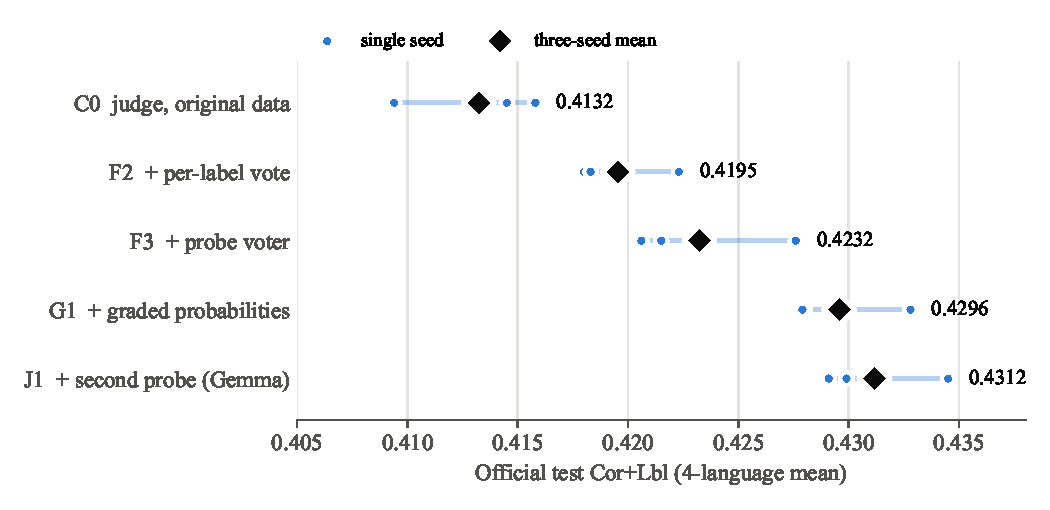
\includegraphics[width=0.85\textwidth]{images/test_seeds.pdf}
    \caption{Official test Cor+Lbl for each training seed (dots) and the three-seed mean (diamond). Every component improves every seed; the weakest J1 seed (0.4291) is well above the strongest C0 seed (0.4158).}
    \label{fig:test}
\end{figure}

\begin{itemize}
    \item \textbf{Test agrees with validation.} The order C0 $<$ F2 $<$ F3 $<$ G1 $<$ J1 holds on test as on val\_select. The increments up to G1 are about the same size; the last one, from the second probe, is about half its validation size ($+0.0016$).
    \item \textbf{Final gain.} The final detector gains $+0.0180$ Cor+Lbl over C0, about five times the seed standard deviation of C0.
    \item \textbf{Consistency.} The gain is positive for each of the three seeds and each of the four languages, $+0.014$ to $+0.021$ per language. All twelve seed--language pairs improve.
    \item \textbf{Mechanism.} IoU rises by 0.021 through the vote and the probes, and Cor by 0.015, mostly through the graded probabilities.
    \item \textbf{Against the shared-task entry.} The gain is $+0.034$ Cor+Lbl, of which $+0.016$ comes from the reimplementation and the decoder fix (C0) and $+0.018$ from the uncertainty components.
\end{itemize}

\paragraph{Leaderboard.}
The SHROOM-Visions leaderboard stayed open after the competition and lists each team's best submission per language. Table~\ref{tab:leaderboard} shows where the final detector stands on it.
\begin{itemize}
    \item \textbf{Position of G1.} After our G1 submissions, the SmurfCat team was 5th in English, French and Italian and 2nd in Chinese, as of 15~November~2026. All four entries came from one submission, G1 with seed 123, and not from a mix of systems per language.
    \item \textbf{Position of J1.} J1 with seed 123 is above G1 seed 123 in all four languages, so it is now our best entry in each. Against the other teams of that snapshot, it would rank 5th, 5th, 4th and 2nd: in Italian it passes the team that was 4th (0.4315 against 0.4295).
    \item \textbf{Seed mean.} Seed 123 is the best of the three seeds, so its position is optimistic. The three-seed mean of J1, which is our test claim, would rank 5th, 5th, 5th and 2nd.
    \item \textbf{Official ranking.} The ranking in the task overview~\cite{vazquez2026shroomvisionsoverview} was fixed at the evaluation deadline. It still lists our shared-task entry at 8th, 6th, 7th and 5th.
\end{itemize}

\begin{table}[!htb]
    \centering
    \caption{Position on the SHROOM-Visions Cor+Lbl leaderboard (29 entries for English, 22--23 for the other languages; snapshot of 15~November~2026). ``Team above'' and ``Team below'' are the other teams ranked directly above and below G1 seed 123 in that snapshot; the J1 ranks are computed against the same snapshot.}
    \label{tab:leaderboard}
    \resizebox{\textwidth}{!}{%
    \begin{tabular}{lcccc}
    \toprule
     & en & fr & it & zh \\
    \midrule
    1st place & 0.4336 & 0.4738 & 0.4511 & 0.5040 \\
    Team above & 0.3943 & 0.4440 & 0.4295 & 0.5040 \\
    Team below & 0.3879 & 0.4071 & 0.4213 & 0.4845 \\
    \midrule
    Our shared-task entry (official ranking) & 0.3516 (8th) & 0.3968 (6th) & 0.3926 (7th) & 0.4564 (5th) \\
    G1 seed 123 (leaderboard, 15 Nov.) & 0.3920 (5th) & 0.4237 (5th) & 0.4286 (5th) & 0.4870 (2nd) \\
    J1 seed 123 (would rank) & 0.3927 (5th) & 0.4264 (5th) & 0.4315 (4th) & 0.4874 (2nd) \\
    J1 three-seed mean (would rank) & 0.3921 (5th) & 0.4218 (5th) & 0.4258 (5th) & 0.4851 (2nd) \\
    \bottomrule
    \end{tabular}}
\end{table}

Our Cor is still well below that of the top teams: in English it is 0.4560 (J1 seed mean) against 0.5534 for the winner. The remaining gap is mostly in how well the probabilities rank characters, not in where the spans are.

\section{Summary of decisions}

Table~\ref{tab:decisions} lists every validation-based decision of the program in the order in which it was made. Together they used 28 candidate evaluations on val\_select. No decision compared more than five candidates, and none was reopened.

\begin{table}[!htb]
    \centering
    \caption{Decision log. All choices were made on val\_select; val\_confirm only re-checked them.}
    \label{tab:decisions}
    \resizebox{\textwidth}{!}{%
    \begin{tabular}{llll}
    \toprule
    Decision & Question & Candidates & Choice \\
    \midrule
    D1 & judge backbone & Qwen3-VL-8B, Gemma-3-12B, InternVL3-8B, Pixtral-12B & Qwen3-VL-8B \\
    D2 & synthetic pilot (old decoder) & C1, C4, C4x & none promoted \\
    D3 & vote threshold, single-label vote & $k \in \{2, 3, 4\}$ & $k = 3$ \\
    D2b & synthetic re-check (new decoder) & C1, C4, C4x & none promoted \\
    D3\_3a2 & vote threshold, per-label vote & $k \in \{2, 3, 4\}$ & $k = 3$ \\
    D2c & prior-matched synthetic & C4x-b, C1-b & none promoted \\
    D4 & integration & F1 = C0, F2, F3, F4 & F3 \\
    D6 & probability output (post-hoc) & G0, G1, G2 & G1 \\
    D7 & second probe judge (post-hoc) & J0 = G1, J1, J2 & J1 \\
    \bottomrule
    \end{tabular}}
\end{table}
